\section{Evaluation}
\label{sec:evaluation}


\iffalse
%We prove the correctness and liveness of \sys in Appendix~\ref{appx:proof}.
We summarize the key findings as follows:

%Our evaluation centers around four aspects:

\parab{Scalable throughput.}\sys achieves throughput close to the underlying hardware limit, and scales linearly to 1K hosts.

\parab{Low latency.}With reconfigurable chip, \sys adds less than 5$\mu$s to one-way delay for 1K hosts. With switch CPU, \sys adds less than 15$\mu$s delay.

\parab{Low network and CPU overhead.}\sys's beacons only consume 0.3\% link capacity. At switches, beacon packets can be processed by a CPU core.

\parab{Fast failure recovery.}

%\parab{Resilient to background traffic.}\sys is adaptive to delay variance in the network by re-synchronizing clocks. Hence, \sys can share the network fairly with background TCP traffic.

\parab{Improve application throughput.} Compared to locking, \sys{} improves throughput by 50x for a transactional key-value store.
\fi

\subsection{Methodology}
\label{sec:testbed}

Our testbed has 32 servers and 10 Arista 7060CX 100G switches~\cite{arista}, forming a 3-layer fat-tree topology (4 ToR, 4 Spine, and 2 Core) similar to Figure~\ref{fig:dcn}.
Each server has 2 Xeon E5 CPUs and a Mellanox ConnectX-4 NIC. %running RoCEv2~\cite{infinibandrocev2}.
We dedicate a CPU core as representative of each switch and NIC to process beacons (Sec.\ref{sec:end-host}). The host representative is directly connected to the switch, so beacon packets do not need encapsulation.
Because we only have one switch with Barefoot Tofino~\cite{tofino} reconfigurable chip, we only use it for microbenchmarks.
%We use the second testbed in most benchmarks because it has larger scale.
%We use a testbed of 8 Dell R720/R730 servers and 10 Arista 100G Ethernet switches~\cite{arista} to benchmark the efficiency of \sys. %The topology is similar to Figure~\ref{fig:dcn}.
%Each server is equipped with two Xeon E5 CPUs and one Mellanox ConnectX-4 NIC. Because we have not found a low latency interface in the switch OS to process beacon packets, we connect one Dell R720 server with Mellanox ConnectX-3 NICs to each of the switches to mimic the switch CPU. %Since the bottleneck in our benchmarks is the CPU instead of the network, there is unlikely to be congestion loss.
%Performance using data-plane programmable switches are expected to be better, but not evaluated because we do not have such a switch.
In small-scale experiments (1$\sim$32 processes), each process runs on a distinct server. Each process uses a pair of threads for sending and receiving, respectively.
For experiments with 64$\sim$512 processes, each server hosts the same number of processes.
%With 16 processes per NIC, the throughput of NICs is saturated.
Clocks are synchronized via PTP~\cite{correll2005design} every 125 ms, achieving an average clock skew of 0.3~$\mu$s (1.0~$\mu$s at 99\% percentile), which agrees with Mellanox's whitepaper~\cite{mellanox-ptp}.
We choose beacon interval to be 3~$\mu$s.


\iffalse
\begin{table}[t]
\centering
\scalebox{0.85}{
\begin{tabular}{|l|r|r|r|r|r|r|}
\hline
Servers & \multicolumn{3}{c|}{Num switches} & \multicolumn{3}{c|}{Num downlinks} \\
\hline
Host & ToR & Leaf & Core & ToR & Leaf & Core \\
\hline
2        & 1 & 0 & 0 & 2 & 0 & 0 \\
\hline
4    & 2 & 2 & 0 & 2 & 2 & 0 \\
\hline
8    & 4 & 4 & 2 & 2 & 2 & 4 \\
\hline
64    & 8 & 4 & 2 & 8 & 4 & 4 \\
\hline
1024  & 64 & 16 & 8 & 16 & 16 & 16 \\
\hline
\end{tabular}
\vspace{-10pt}
}
\caption{Network topologies for evaluation.}
\label{tab:eval-topology}
\end{table}

We evaluate 5 different system scales in Table~\ref{tab:eval-topology}: testbed consisting of one to three layers of network switches, as well as simulation of three-layer fat-tree topology with 64 or 1024 hosts.
Topologies in Table~\ref{tab:eval-topology}.
For large-scale experiments, we use NS-3~\cite{henderson2008network} for simulation.
The link bandwidth, link delay and processing delay are extracted from three-layer testbed experiments.
To make simulations faster, each sender only sends one message to a randomly chosen receiver.
\fi

\iffalse
\begin{figure*}[t!]
	\begin{minipage}{.31\textwidth}
    	\centering
		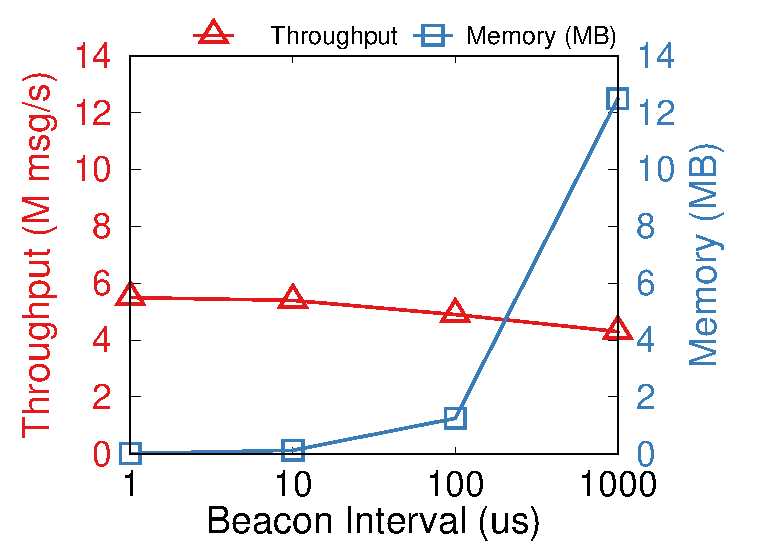
\includegraphics[width=\textwidth]{gnuplot/reorder_receiver.eps}
		\caption{Reordering CPU and memory overhead on hosts.}
		%\label{fig:reorder-overhead}

		%\centering
		%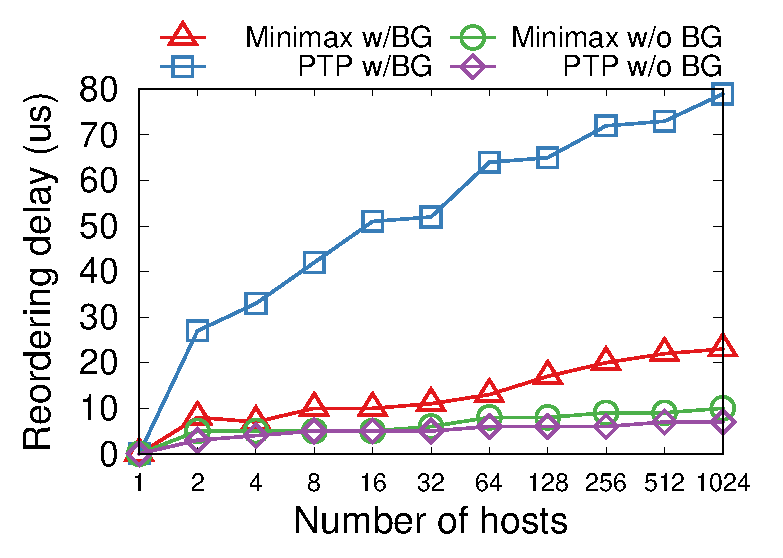
\includegraphics[width=\textwidth]{gnuplot/reordering_delay.eps}
		%\caption{Reordering delay with clock synchronization methods and background traffic (BG).}
		%\label{fig:clock-sync}
	\end{minipage}
    \hspace{0.01\textwidth}
    \begin{minipage}{.31\textwidth}
    	\centering
		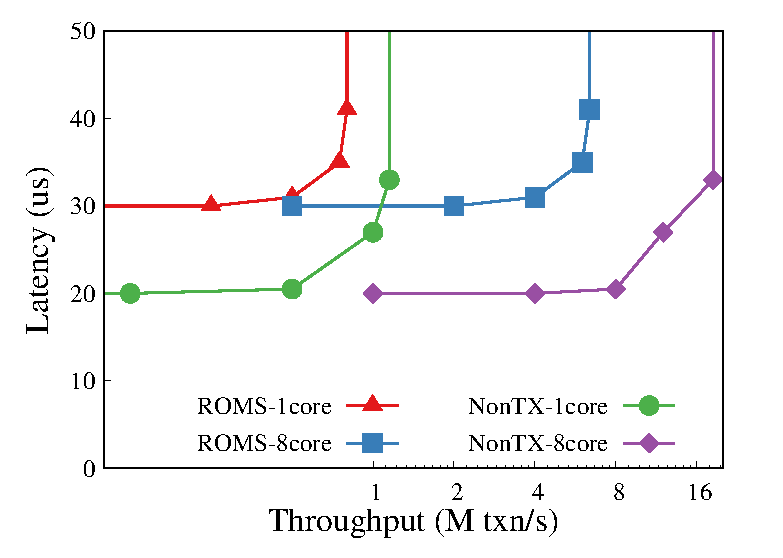
\includegraphics[width=\textwidth]{gnuplot/ycsb.eps}
		\caption{Throughput and latency of YCSB+T transactional key-value stores.}
		\label{fig:ycsb}

		\centering
		%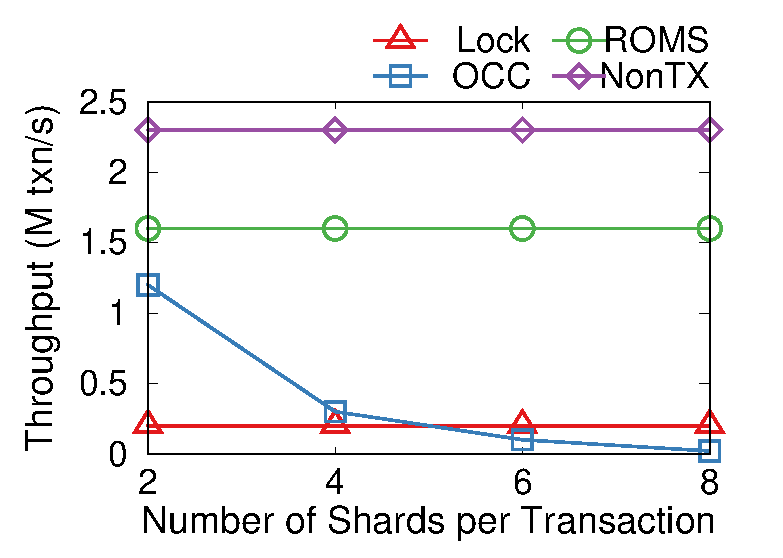
\includegraphics[width=\textwidth]{gnuplot/multishard.eps}
		\caption{Throughput of multiple keys per transaction.}
		\label{fig:multishard}
    \end{minipage}
	\hspace{0.01\textwidth}
	%\begin{minipage}{.31\textwidth}
	%	\centering
	%	\subfloat[Throughput.\label{fig:loss-throughput}]
	%	{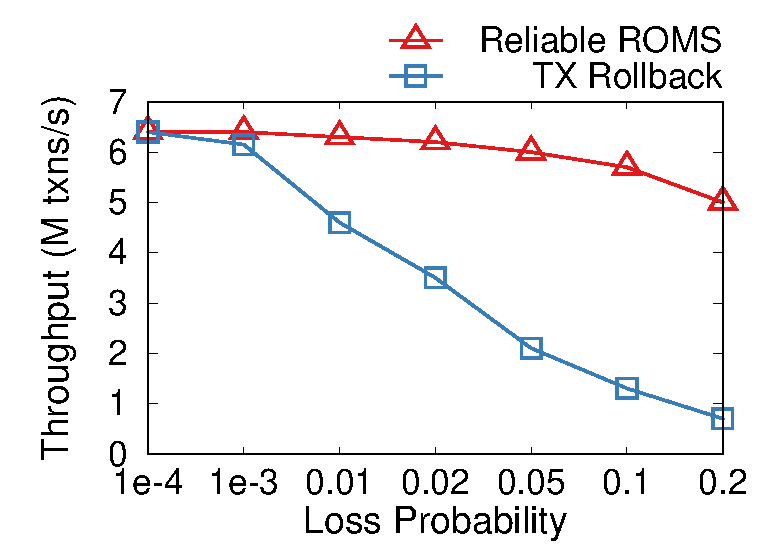
\includegraphics[width=\textwidth]{gnuplot/loss_tput.eps}}
	%	\vspace{0.01\textwidth}
	%	\subfloat[Latency.\label{fig:loss-latency}]
	%	{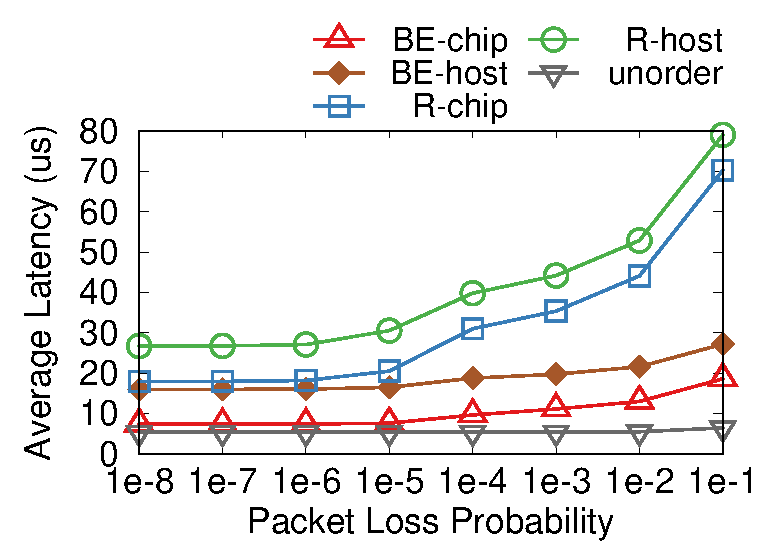
\includegraphics[width=\textwidth]{gnuplot/loss_latency.eps}}
	%	\caption{Comparison of reliable \sys and application-layer transaction rollback.}
	%	\label{fig:ycsb-loss}
	%\end{minipage}
\vspace{-15pt}
\end{figure*}
\fi

\subsection{Microbenchmarks}

\parab{Scalability.}
Figure~\ref{fig:total-order} compares the scalability of \sys{} with other total order multicast algorithms using token~\cite{rajagopalan1989token}, Lamport timestamp~\cite{lamport1978time}, and centralized sequencer at programmable switch~\cite{eris} or host NIC~\cite{kaminsky2016design}.
Each process broadcasts messages to all processes.
\sys{} scales linearly to 512 processes, achieving 5M messages per second per process.
The throughput of \sys is limited by CPU processing and RDMA messaging rate.
Reliable (R) \sys{} has 25\% lower throughput than best effort (BE) \sys{} due to 2PC overhead.%\footnote{Lamport timestamp and token imply reliability. However, our sequencer implementation only provides best effort delivery.}
Reconfigurable chip and host representative deliver the same high throughput (not shown) because we decouple message forwarding from barrier propagation.

%\RED{Compare with optimized Lamport timestamp where received timestamps are exchanged per interval. Optimized Lamport timestamp has a trade-off between latency and throughput. e.g. use 50\% throughput for timestamp exchange: 2.5M msg/s, 512 processes, 5K msg/s, interval = 1/5K = 200 us.}

In contrast, the sequencer is a central bottleneck and introduces extra network delays to detour packets.
The latency soars when throughput of sequencer saturates and congestion appears.
Token shows consistent low throughput because only one process may send at any time.
We apply a common optimization to Lamport timestamp~\cite{lamport1978time} which exchanges received timestamps per interval rather than per message.
It has a trade-off between latency and throughput, \textit{e.g.}, for 512 processes, even if 50\% throughput is used for timestamp exchange, the interval is as high as 200$\mu$s.





\parab{Message delivery latency.}
Figure~\ref{fig:reorder-testbed} shows the average message delivery latency of best effort (BE) and reliable (R) \sys{}.
Best effort \sys{} with reconfigurable chip delivers the smallest latency overhead than unordered delivery. The overhead (1.7$\sim$2.3$\mu$s) is almost constant with different number of network layers and processes, which is half of beacon interval plus clock skew. In contrast, end host representatives introduce extra forwarding delay from the switch to the end host. In our testbed, $\le$8, 16, and $\ge$32 processes have 1, 3, and 5 network hops, respectively.
Reliable \sys{} adds an RTT to best effort \sys{} due to Prepare phase in 2PC.
The RTT and host forwarding delay are proportional to network hop count.

As Sec.\ref{subsec:abstration} discussed, packet loss rate of links are typically lower than $10^{-8}$, but faulty links may have loss rates above $10^{-6}$.
We simulate random message drop in \textit{lib1pipe} sender and receiver to evaluate how packet loss affects latency in the testbed with 512 processes.
As Figure~\ref{fig:reorder-loss} shows, when loss rate is higher than $10^{-5}$, latency of \sys{} starts to grow. In both BE- and R-\sys{}, a lost beacon packet on any link will stall delivery of barrier until the next beacon, and all receivers need to wait for the worst link. In R-\sys{}, a lost message in prepare phase will trigger retransmission, which will stall the network for an RTT. So, R-\sys{} is more sensitive to packet loss.
Packet loss has almost no impact on throughput because \sys{} can transfer new messages while retransmitting lost packets.
Besides packet loss, queuing delay caused by background traffic can also increase \sys{} latency. With 10 background TCP flows per link, latency inflation of BE-\sys{} and R-\sys{} latency are 30~$\mu$s and 50~$\mu$s, respectively.

%\textbf{Reordering delay (Y) - background flows per link (X); cluster scale (lines): experimentation.}

%\RED{The beacon interval is not amplified by network layers, because the algorithm synchronizes beacon arrival times. doesn't make sense}
%For the three-layer topology, a larger number of hosts slightly increases reordering delay.

%Figure~\ref{fig:reorder-simulation} shows how minimax clock synchronization adapts to imbalanced link or host delays. We simulate two senders and two receivers connected via 4 links. When one sender $S_1$ has 10~$\mu$s more delay due to background traffic, minimax clock synchronization adjusts the sender's timestamp to preserve minimal reordering delay, while physical clock synchronization does not account for the different sender delays. When one network link $S_2 \rightarrow R_2$ has 100~$\mu$s more delay, due to multi-path, both synchronization mechanisms have more reordering delay. When two links $S_2 \rightarrow R_1$ and $S_2 \rightarrow R_2$ both have 10~$\mu$s more delay, minimax clock synchronization can compensate the change.


\parab{Failure recovery.}
Figure~\ref{fig:failure-recovery} depicts failure recovery time, which measures the average time of barrier timestamp stall for correct processes.
In our testbed, a failure is detected if beacon is not received for 10 beacon intervals (30~$\mu$s).
In addition to failure detection time, the recovery procedure in Sec.\ref{sec:reliable} requires 6 network diameters plus the time to transmit and process messages.
Core link and switch failures do not affect connectivity, so, only the controller needs to be involved, and no process is considered to be failed.
Host, NIC, host link, and ToR switch failures cause processes to disconnect from the system, so, the recovery takes longer because each correct process needs to discard messages from or to them.


%\begin{figure}[t]
%\centering
%
\includegraphics[width=0.48\textwidth]{images/fixme.pdf}
%\caption{CDF of end-to-end delay and reordering delay.}
%\label{fig:cdf-delay}
%\end{figure}


\begin{figure}[t]
	\centering
	\subfloat[CPU processing overhead.\label{fig:cpu-overhead}]
	{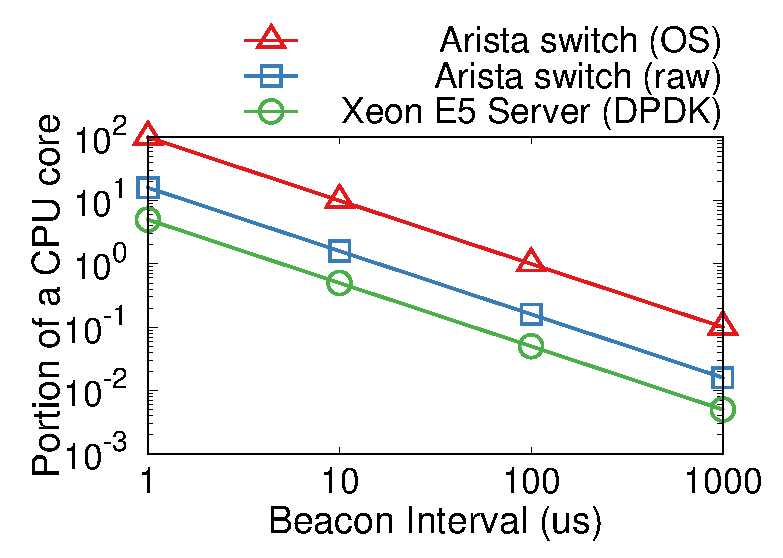
\includegraphics[width=0.22\textwidth]{gnuplot/beacon_cpu_overhead.eps}}
	\hspace{0.01\textwidth}
	\subfloat[Network bandwidth overhead.\label{fig:network-overhead}]
	{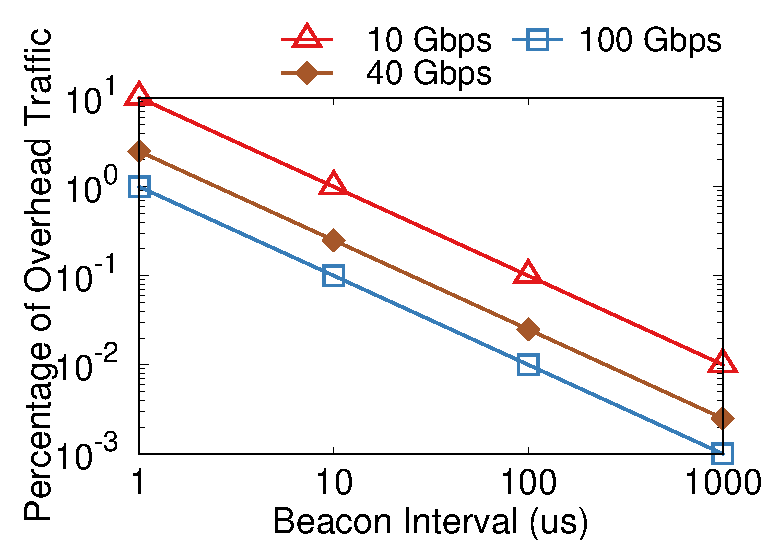
\includegraphics[width=0.22\textwidth]{gnuplot/beacon_network_overhead.eps}}
	\caption{
		Beacon overhead under different beacon intervals.
		CPU processing overhead for Arista switch is extrapolated.
	}
	\label{fig:overhead}
\end{figure}


\parab{CPU overhead.}
The CPU overhead of \sys has two parts: reordering at receivers and beacon processing at switches.
As Figure~\ref{fig:reorder-overhead} shows, the maximal buffer size required on the receiver increases linearly with beacon interval, but only takes a few megabytes. The message delivery throughput degrades slightly with more messages to reorder.

Figure~\ref{fig:cpu-overhead} shows the number of cores required for beacon processing of a 32-port switch.
A host CPU core can sustain 3~$\mu$s beacon interval of the switch, which is our testbed setting.
If switch CPUs are used instead, the raw packet processing capacity of a switch CPU is roughly 1/3 of a host CPU core.
If we can bypass the kernel network stack and process packets efficiently at Arista switches, a single switch CPU core can sustain 10~$\mu$s beacon interval.


\parab{Network overhead.}
As Figure~\ref{fig:network-overhead} shows, with high link bandwidth and a reasonable beacon generation interval (\emph{e.g.} 3~$\mu$s), beacon traffic is a tiny portion (\emph{e.g.} 0.3\%) of link bandwidth. Because beacons are hop-by-hop, the overhead is only determined by the beacon interval and does not increase with system scale.


%Figure~\ref{fig:clock-sync} compares reordering delay of minimax clock synchronization with physical clock synchronization (PTP). Without background traffic, minimax clock synchronization achieves similar accuracy with PTP. In the presence of background TCP traffic, physical clock synchronization leads to high reordering delay, while \sys adapts to variable congestion delay.

\iffalse
\subsubsection{Incremental Deployment}
\label{sec:eval-incremental}


\begin{figure}[t]
\centering
        \subfloat[Clock convergence.\label{fig:clock-convergence}]
        {
\includegraphics[width=.23\textwidth]{images/fixme.pdf}}
        \hspace{0.01\textwidth}
        \subfloat[Reordering delay.\label{fig:incremental-delay}]
        {
\includegraphics[width=.23\textwidth]{images/fixme.pdf}}
\caption{[Simulation] Merging two running TOMS systems by adding a network link between them.}
\label{fig:incremental}
\end{figure}

Figure~\ref{fig:clock-convergence} shows
Converge time graph, compare with physical time synchronization solution

Figure~\ref{fig:incremental-delay} shows the reordering delay. (spike then fall back)
\fi
